\section{BULUT VERİ DEPOLAMA VE GİZLİLİK YÖNETİMİ}

Bu bölümde FaceScan AI projesinin veri depolama mimarisi, gizlilik kararları ve bunların bulut tasarımına etkileri ele alınmaktadır.

\subsection{Tarayıcı Yerel Depolama ile Veri Tabanı Maliyeti Eliminasyonu}

Bulut tabanlı veri tabanları (AWS DynamoDB, Google Firestore, MongoDB Atlas vb.), veri okuma/yazma işlemleri başına talep ücreti uygulamakta ya da depolanan veri miktarına bağlı aylık ücretlendirme içermektedir. FaceScan AI projesinde bu maliyet kalemini tamamen ortadan kaldırmak için kullanıcıya ait tarama geçmişi verileri \textbf{tarayıcının yerel depolama alanı (LocalStorage)} üzerinde saklanmaktadır.

LocalStorage, HTML5 standardıyla tanımlanmış olan ve tarayıcı bazında birbirinden izole çalışan bir anahtar-değer depolama mekanizmasıdır. Kullanıcının her tarama kaydı, tarih zaman damgasını (timestamp), teşhis puanlarını ve renk analiz sonuçlarını içeren bir JSON nesnesi olarak serileştirilmekte ve LocalStorage'a yazılmaktadır:

FaceScan AI'ın veri gizliliği modeli üç temel prensip üzerine kurulmuştur:
\begin{itemize}
  \item \textbf{Veri Minimizasyonu:} Yalnızca analiz sonuçları saklanmakta; ham görüntü verileri hiçbir aşamada kalıcı olarak depolanmamaktadır.
  \item \textbf{Yerel Kalma (Data Residency):} Tüm kişisel sağlık verileri kullanıcının kendi cihazında kalmakta; bulut sunucularına aktarılmamaktadır.
  \item \textbf{Kullanıcı Kontrolü:} Kullanıcı, tarama geçmişini uygulama içinden tamamen silebilmektedir.
\end{itemize}

Bu model, Avrupa Birliği GDPR (Genel Veri Koruma Tüzüğü) ve Türkiye KVKK (Kişisel Verilerin Korunması Kanunu) kapsamındaki "veri minimizasyonu" ilkesiyle örtüşmektedir. Kullanıcının yerel depolama üzerinde saklanan tarama geçmişi, Şekil \ref{fig:bulut_dashboard}'de gösterilen Dashboard ekranındaki "Geçmiş Analizler" listesi aracılığıyla yönetilmektedir. Herhangi bir taramanın ayrıntılarına tıklandığında, Şekil \ref{fig:bulut_detaylar}'de sunulan detay ekranı açılmakta ve veriler yerel bellekten okunarak dinamik olarak oluşturulmaktadır. Bu sayede hiçbir kullanıcı verisi uzak sunuculara gönderilmemekte, bulut altyapısı üzerindeki işlem ve ağ trafiği yükü minimize edilmektedir.

\begin{figure}[h!]
    \centering
    \begin{subfigure}[b]{0.45\linewidth}
        \centering
        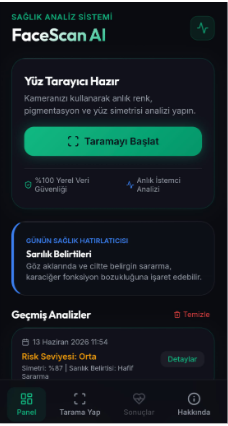
\includegraphics[width=\linewidth]{sekil2_dashboard.png}
        \caption{Geçmiş Analizler Listesi}
        \label{fig:bulut_dashboard}
    \end{subfigure}
    \hfill
    \begin{subfigure}[b]{0.45\linewidth}
        \centering
        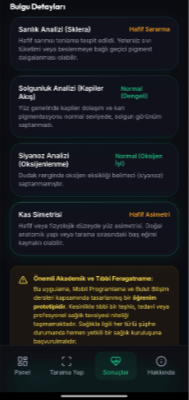
\includegraphics[width=\linewidth]{sekil6_detaylar.png}
        \caption{Yerel Veriden Üretilen Detaylar}
        \label{fig:bulut_detaylar}
    \end{subfigure}
    \caption{FaceScan AI -- Yerel Depolama (LocalStorage) Entegrasyonu ve Veri Yönetimi}
    \label{fig:bulut_veri_yonetimi}
\end{figure}


\subsection{Hibrit Mobil Entegrasyon ve Bulut Köprüsü}

Uygulama, yalnızca bir web sayfası olarak değil, Android cihazlarda yerel uygulama görünümüyle çalışan hibrit bir paket olarak da sunulmaktadır. Bu hibrit model, Trusted Web Activities (TWA) standardını kullanmaktadır. TWA uygulamaları, Chrome tarayıcısı üzerinden bulut adresine köprü kurarak çalıştığından, yerel cihazdaki APK dosyasının her güncellenmesine gerek kalmadan buluttaki web uygulaması güncellendiğinde değişiklikler otomatik olarak tüm kullanıcılara yansımaktadır.

Bu yaklaşım, geleneksel yerel uygulama güncelleme süreçlerine (Google Play Store onay süreci, ortalama 1-3 günlük bekleme) kıyasla anlık güncelleme kapasitesi sunmakta ve bulut altyapısının hız avantajını doğrudan mobil deneyime yansıtmaktadır. Bulut üzerinde çalışan web uygulamasının istemci tarafındaki yetenekleri, WCAG 2.1 erişilebilirlik standartları, hibrit Android paketi (.apk) indirme kanalları ve güvenlik tarama raporları uygulamanın "Hakkında" (Info) sekmesi altında doğrudan sunulmaktadır (Bkz. Şekil \ref{fig:bulut_hakkinda}). Bu sayede, bulut platformunda yapılan en güncel iyileştirmeler (güvenlik yamaları, erişilebilirlik güncellemeleri vb.) anında TWA tabanlı istemciye yansımakta ve indirme bağlantıları doğrudan güncel kalmaktadır.

\begin{figure}[h!]
    \centering
    \begin{subfigure}[b]{0.45\linewidth}
        \centering
        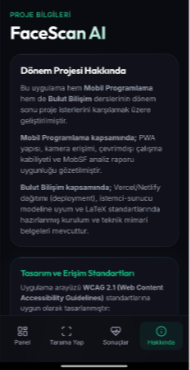
\includegraphics[width=\linewidth]{sekil7_hakkinda_1.png}
        \caption{Hakkında Sekmesi Üst Kısım}
        \label{fig:bulut_hakkinda_1}
    \end{subfigure}
    \hfill
    \begin{subfigure}[b]{0.45\linewidth}
        \centering
        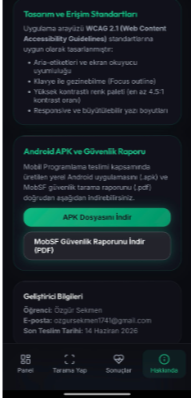
\includegraphics[width=\linewidth]{sekil8_hakkinda_2.png}
        \caption{APK ve Güvenlik Raporu İndirme}
        \label{fig:bulut_hakkinda_2}
    \end{subfigure}
    \caption{FaceScan AI -- Bulut Altyapısı Bilgilendirme ve Varlık Dağıtım Arayüzü}
    \label{fig:bulut_hakkinda}
\end{figure}

